In this chapter, you will learn how to make
free-standing wheat sourdough bread.

\begin{figure}[!htb]
  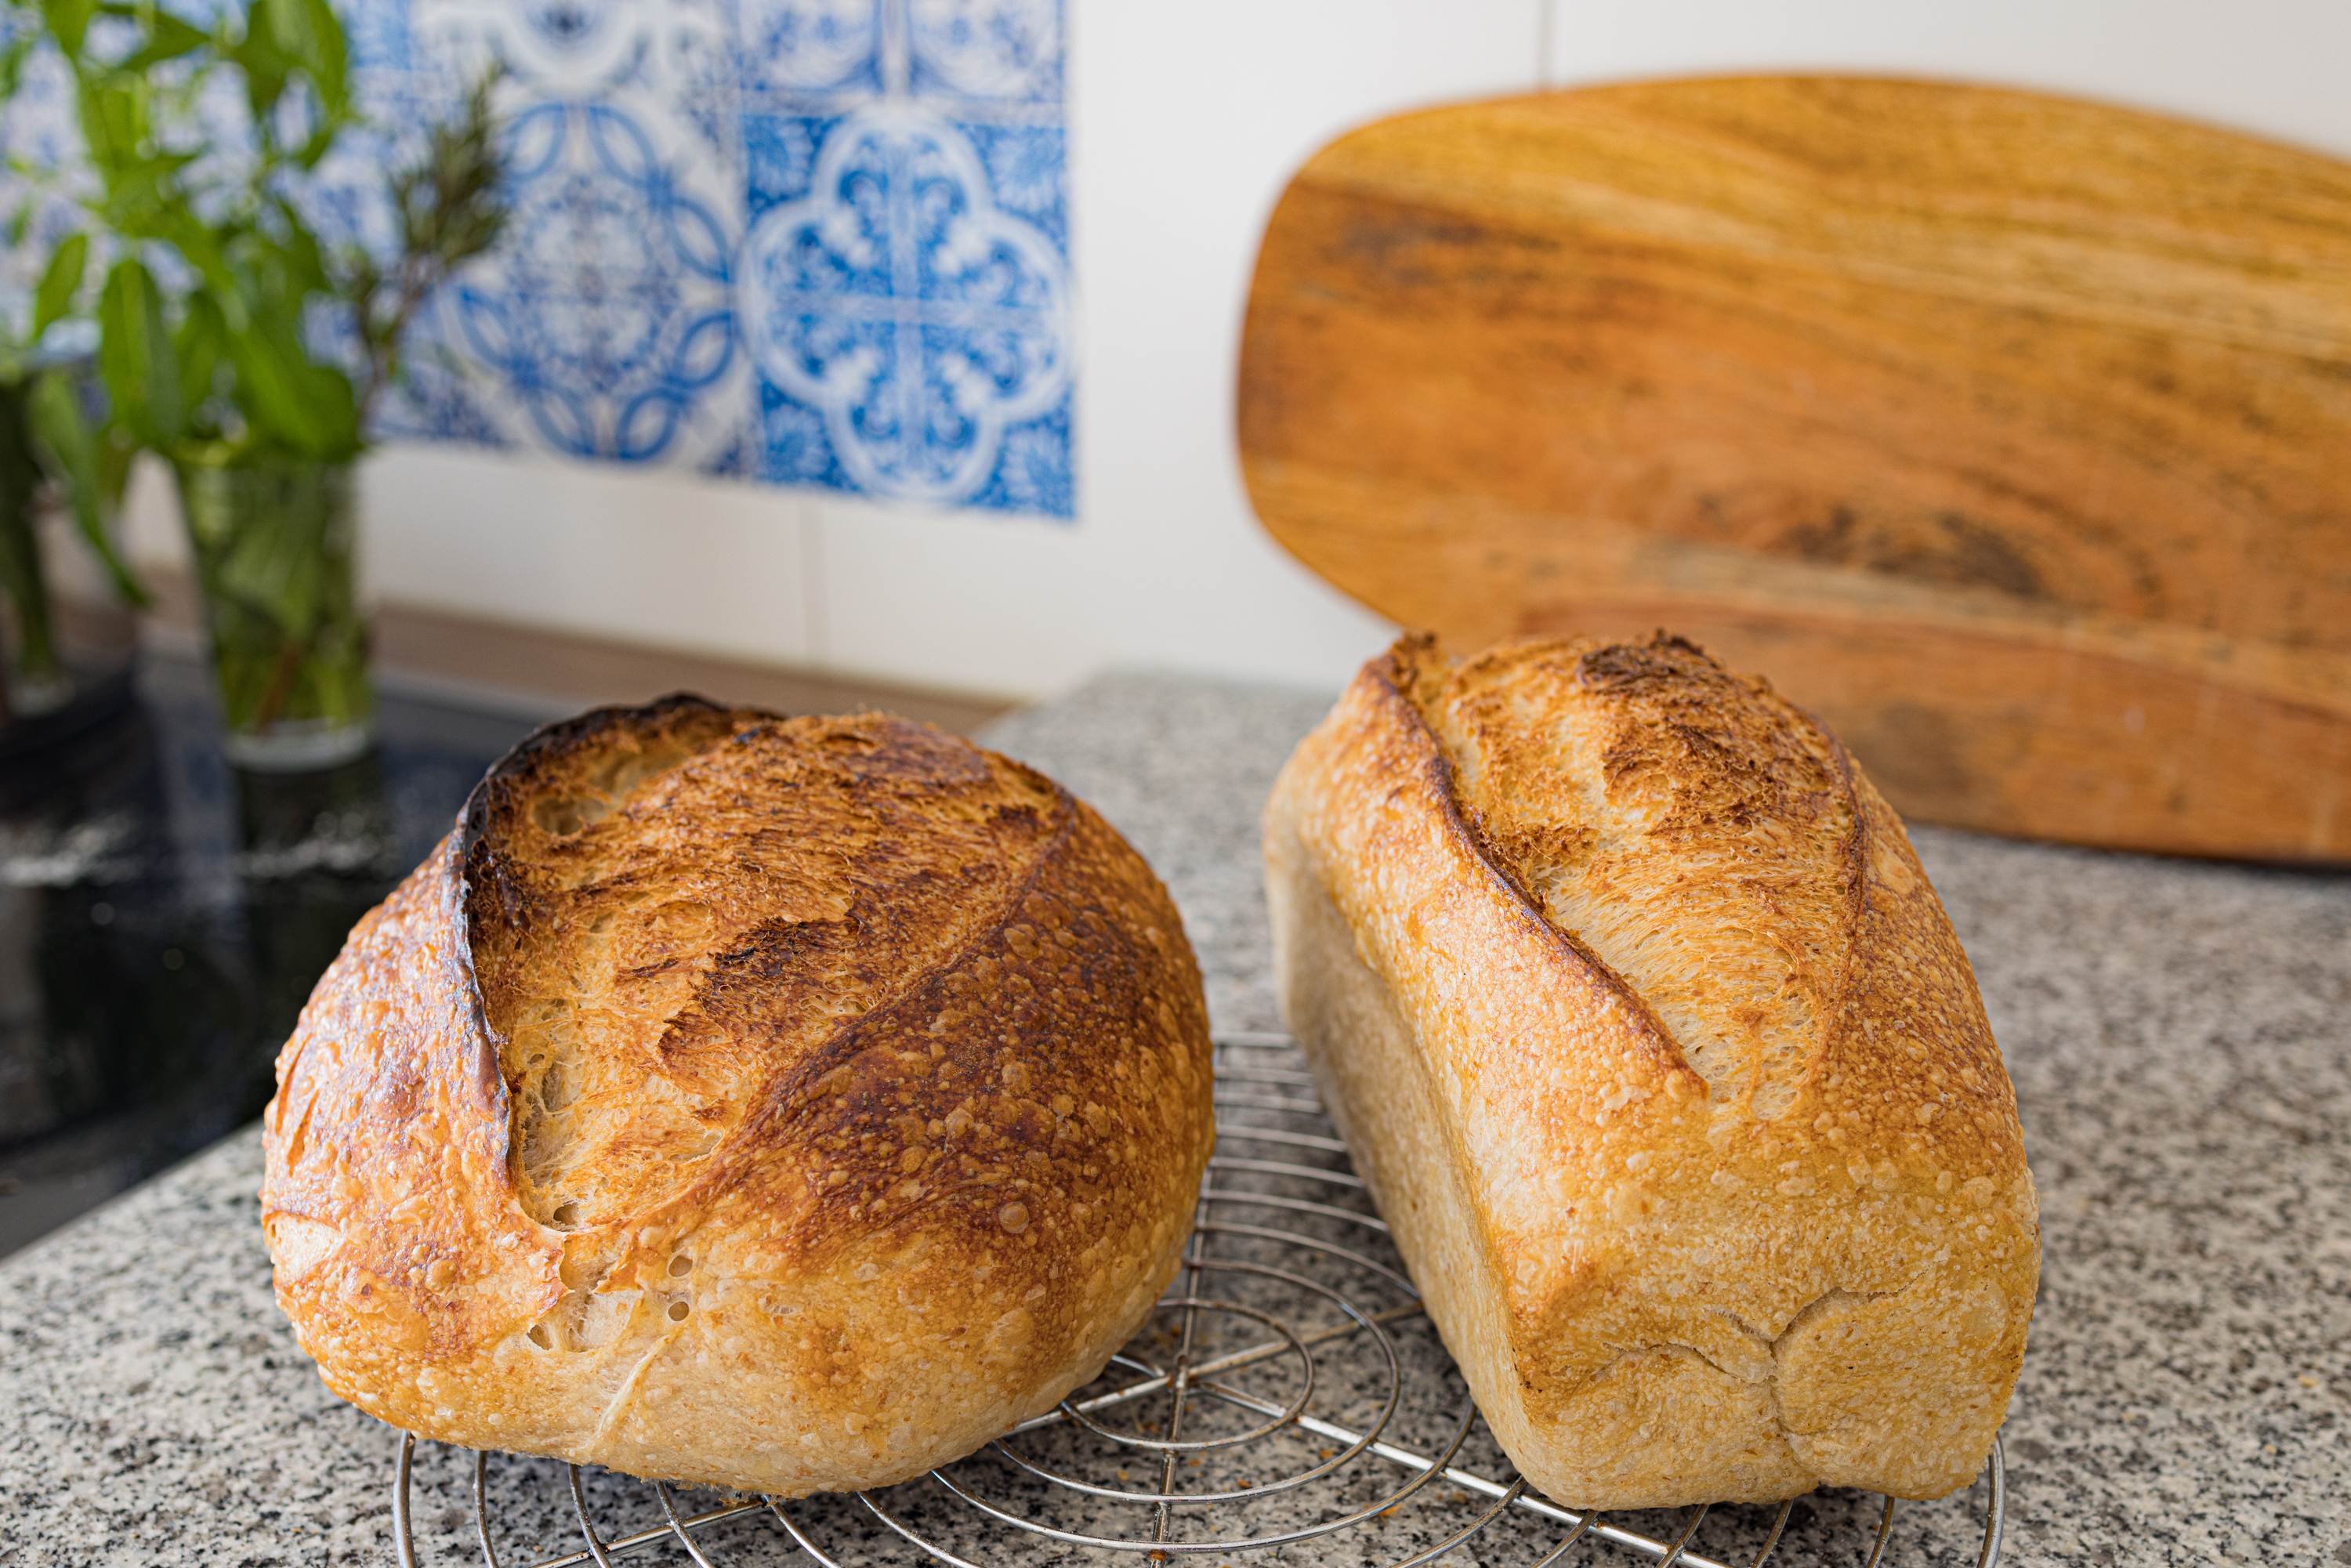
\includegraphics[width=\textwidth]{loaf-pan-free-standing.jpg}
  \caption{A free-standing sourdough bread made with wheat flour}
\end{figure}

A free-standing sourdough bread is my favorite
type of bread. It combines a great crunchy crust, superb
flavor, and a soft fluffy crumb. This is the type of bread
that is being inhaled by my friends and family. Unfortunately
making this type of bread requires a lot more effort, patience,
and technique than other types of bread. You have to perfectly
balance the fermentation process. You can not ferment for too
short and also not for too long. The techniques you need to
learn require a bit more skill. It took me several attempts
to get this right. One of the challenges I faced was that
I had the wrong flour. I didn't properly know how to use my oven.
When should I stop the fermentation? There is a lot of information
out there. I dug through most of it and have tried almost everything.
In many cases the information was wrong, in other cases, I
found another valuable puzzle piece. Aggregating all this
information was one of my main motivations to start the bread code.
My key learning was that there there is no recipe that
you can blindly follow. You will always have to adapt the recipe
to your local available tools and environment.

But do not worry. After reading this chapter you will know
all the signs to look out for. You will be able to read your dough.
You will turn into a confident hobby baker that can bake bread
at home, at high altitudes, at low altitudes, in summer, in winter,
at your friend's place, and even on vacation. Furthermore,
you will know how to scale your production from 1 bread to 100 loaves of bread.
If you ever wanted to open up a bakery, consider this knowledge to
be your foundation.

Mastering this process will enable you to bake amazing bread without
ever buying yeast again.

\section{The process}

\begin{figure}[!htb]
  \includegraphics[width=\textwidth]{sourdough-process-overview.jpg}
  \caption{An overview of the whole sourdough process from start to finish}
\end{figure}

The whole process of making great sourdough bread starts with
readying your sourdough starter. The key to mastering
this process is to manage the fermentation process properly.
For this, the basis is to have an active and healthy
sourdough starter.

Once your starter is ready you proceed to mix all the ingredients.
You want to homogenize your sourdough starter properly. This
way you ensure an even fermentation across your whole dough.

After a short break, you will proceed and create dough strength.
Kneading will create a strong gluten network. This is essential
to properly trap the CO2 created during the fermentation.

Once you kneaded the bulk fermentation starts. Bulk fermentation
because you typically ferment multiple doughs together in one bulk.
Understanding when to stop this step will take some practice.
But nothing to worry about, you will learn the exact signs to look out for.

Once this is completed you need to divide your large blob of
dough into smaller pieces and preshape each piece. This allows
you to apply more dough strength and shape more uniform loaves.

The proofing stage follows where you finish the fermentation process.
Depending on your time you can proof at room temperature or in the fridge.
Mastering proofing will turn your good loaf into a great loaf.

Lastly, you will finish the whole process by baking. You will learn different
options on how to properly steam your dough. This way your
dough will have a beautiful oven spring. During the second
stage of the baking process, you will finish building your crust.

All the steps rely on each other. You will need to get each of
the steps right to make the perfect bread.

\section{Readying your starter}

The most crucial part of the bread-making process is your starter.
The starter is what starts the fermentation in your main dough.
If your starter is off, then your main dough is also going
to cause trouble during the fermentation. Your starter's
properties are passed on to your main dough. If your starter
doesn't have a good balance of yeast to bacteria, so will your
main dough.

\begin{figure}[!p]
  \centering
  \includegraphics[width=\textwidth]{1-ready-starter}
  \caption[Readying a starter]{A flowchart showing how you can prepare your starter before baking.
  This assumes you are using a stiff starter.}
\end{figure}

Generally, think of the dough you are mixing as a big starter with salt.
After mixing all the ingredients you have a green field environment again.
The yeast and bacteria start to fight again to outcompete each other.
There is plenty of food available and they all do their best to win.
Depending on the starter you mix into your dough some of the microorganisms
might have an advantage over the others.

The first option to achieve a good balance is to apply feedings.
If your starter hasn't been fed in a long period the
bacteria dominate. This happens if your starter has been
sitting unused in the fridge for instance. As more and more
acidity piles up the environment is becoming more and more hostile
to the yeast. The lactic acid bacteria tolerate this environment
better. Your dough fermentation would be more towards the
bacterial side with this starter. By applying a couple of
feedings the yeast becomes more active. The older your
starter the more acid resistant the yeast becomes. Initially,
I had to feed my starter 2-3 times to fix the balance. With my
more mature starter, one feeding seems to be enough to balance
the microorganisms.

Some people use a 1:1:1 ratio to refresh the starter. This would
be one part of the old starter (10g for instance), 1 part of flour,
and one part of water. I think this is utter rubbish. As mentioned
your starter is a gigantic dough. You would never a 1:1:1 ratio to
make a dough. You might use a maximum of 20 percent starter to
make a dough. That's why I advocate using a 1:5:5 ratio or a
1:10:10 ratio depending on how ripe your starter is. As I almost
always use a stiffer sourdough starter due to its enhanced
yeast fermentation advantages (see section \ref{section:stiff-starter})
my ratio is never 1:5:5. My ratio would be 1:5:2.5 (1 part old starter,
5 parts flour, 2.5 parts water). If it is very warm where you live
you could opt for the aforementioned 1:10:5 or 1:20:10. This
way you slow down the ripening of your starter. You can use this
trick too to make starter feeding work with your schedule.
If your starter is typically ready in 6 hours but today you need it
ready later, simply increase how much flour/water you feed your starter.
These are all values that you need to experiment with on your own.
Every starter is unique and might behave slightly differently.

The second option at your disposal is the starter quantity that
you use to make the dough. As previously stated your starter
regrows inside of your main dough. While I would normally use
10-20 percent of starter based on the flour, sometimes I go
as low as 1 percent starter. This way the microorganisms have
more room to balance out while fermenting the dough. If my sourdough
starter has not been fed in a day I might use 5 percent of sourdough
to make a dough.  If I push this to 2 days without feedings
I lower the starter amount even further. I would opt for the
previously mentioned 1 percent starter. If the food is very scarce
your microorganisms will sporulate. They need to regrow again
from the spores they created. In this hibernation state, it takes
longer for them to become fully active again. I have tried
several times to make dough directly out of a dry starter.
I wasn't successful because the fermentation took too long.
The microorganisms had to regrow from spores and then begin
the fermentation. As explained earlier there is a limit to
fermentation times as your dough naturally breaks down.
Furthermore, you want your microorganisms to outcompete
other pathogens contained in the flour. The less starter
you use the easier it is for them to reproduce. A strong
starter will outcompete other germs. While the method of
reducing the starter works, I recommend option one more.
It will reliably create better bread. Option 2 is typically
what I use when I fed my starter in the morning but didn't
manage to make a dough in the evening. I don't want to feed
my starter again the next morning. I would like to make a dough
directly without waiting and thus use less of the very ripe starter.

Over time you will become more accustomed to your starter
and how it behaves. You will be able to read the signs of its
activity and judge its state.

\section{Ingredients}

All you need to make a great sourdough bread is flour water and salt. You
can of course add additional things to your dough such as seeds. I personally
enjoy the hearty taste of whole wheat. Thus I like to add around 20-30 percent
of whole wheat flour to the mix. You could also make this recipe with 100 percent
whole wheat flour directly. In this case look out for a strong whole wheat
flour that is made from flour with higher protein. If you don't like whole
wheat you can omit the flour from the recipe. The added whole wheat flour
contains more enzymes and will thus speed up the whole process.

Especially when getting started I recommend to use a bread flour which
contains more gluten than all purpose or cake flour. This is essential
when trying to bake a free standing loaf with sourdough.

Example recipe for 1 loaf:

* 400g of bread flour
* 100g of whole wheat flour
=> 500g of flour in total

* 300g-450g of room temperature water (60 percent up to 90 percent). More on
this topic in the next chapter.
* 50g of stiff sourdough starter (10 percent)
* 10g of salt (2 percent)

In case you want to make more bread simply increase the quantities based on
how much flour you have. Let's say you have 2000g of flour available. The
recipe would look like this.

* 1800g of bread flour
* 200g of whole wheat flour
=> 2000g of flour, equalling 4 loaves

* 1200g up to 1800g of room temperature water (60 to 90 percent)
* 200g of stiff sourdough starter (10 percent)
* 40g of salt (2 percent)

This is the beauty of baker's math. Simply recalculate the percentages and you
are good to go. If you are unsure about how this works please check out the
full chapter \ref{section:bakers-math} which looks at the topic in detail.


\section{Hydration}

Hydration refers to how much water you use for your flour. When
beginning to make bread I always got this wrong. I followed a recipe from the
internet and my dough never looked like a dough shown in the recipe.
The amount of water your flour requires is not fixed. It depends on the flour
you have.

When a seed gets into contact initially the outer layers soak up the water.
That's why when using whole wheat (still containing these layers) you have to
use a little bit more water.

By forming gluten strands water is absorbed into your dough. The higher the
protein value the more water can be used.

Some bakers like to use a highly hydrated dough to create a fluffier dough.
\footnote{Sometimes it almost feels like a comparison of skill value between bakers. The
more water they can handle, the more skillfull the baker.} The reason for this
is the dough's improved extensibility. The wetter the dough the easier it is
for the dough to be stretched. When you pull it, the dough will hold its
shape. In comparison a very stiff (low hydration) dough will maintain its
shape for a longer period of time. To visualize this think of your extensible
dough as a balloon. The stiff dough is a car tire. The yeast has a much harder
time to inflate the care tire compared to the balloon. That's because the
rubber of the car tire is much more elastic. It requires much more force to
inflate the tire. For this reason an extensible dough will inflate more in the
oven. The loaf will be visually bigger and offer an airier more open crumb structure.

While this might sound great, the high hydration causes several sideffects.

1. Your dough becomes more difficult to handle. Your dough will be stickier
compared to a regular dough.
2. Your dough has to be kneaded for longer in order to build a proper gluten
network.
3. During the fermentation your dough might become too extensible and lose
some of the dough strength. To circumvent this stretch and folds are applied
requiring you to invest a lot more work.
4. Shaping becomes much more of a hassle as the dough is very sticky.
5. The dough can stick to the banneton a lot easier while proofing.
6. If you wait too long during proofing the dough won't have enough strength
left to pull upwards and stay flat.
7. Generally the higher the water content the more bacterial fermentation you
have. Thus a wetter dough will reduce in gluten faster than a stiffer dough.
This is why you have to start the fermentation with a sourdough starter in
perfect shape. Bakers use a process called autolyse to shorten the main
fermentation time to circumvent this.
8. The crumb in the end might be perceived as somewhat sticky. It still
contains a lot of water. Personally I love this crumb, but this is a personal
choice.

To achieve such a high hydration dough it is best to slowly add the water to
your dough. Start with 60 percent hydration, then slowly add a bit more water. Knead
again until the water is absorbed. Repeat and add more water. As your dough
has already formed a gluten network, new water can be absorbed much easier.
You will be surprised by how much water your dough can soak up. By doing so I
was easily able to push a low gluten flour to a hydration of 80 percent. This
is also my method of choice when making a dough now. I keep adding water until
I can feel that the dough has the right consistency. As you bake more bread
you will develop a better look and feel for your dough.

All in all increasing the hydration requires a lot of trial and error. There
is however one option that makes things easier and does not cause such a
headache: Slow fermentation. To slow down the fermentation simply use less
sourdough starter or ferment in a cooler environment.

As explained earlier both the protease enzyme and bacteria break down your
gluten network. So as fermentation progresses your dough will automatically
become more extensible. This is because the rubber layers of your care tire
are slowly converted and eaten. Ultimately your car tire turns into a balloon
that can very easily be inflated.  Ultimately when waiting too long the
balloon will burst. You will have no gluten left anymore and your dough
becomes very sticky. Finding the sweet spot of enough rubber eating and not
too much is what this type of bread is about. But don't worry, after reading
this chapter you will have the right tools at your disposal.

The advantages of slow fermentation can be nicely observed when making a yeast
dough with a fast fermentation (1 percent dry yeast based on the flour). The
crumb of such a dough is never as
open as a dough made with sourdough. Furthermore the protease enzyme
can not do its job within such a short fermentation period.
Large industrial bakeries add active malt which contains a
lot more enzymes. This way the time required to make a dough is shortened. You
will most likely find malt as an ingredient in supermarket bread. It is a
great hack. The baked turbo fermentation bread will feature a relatively dense
and not fluffy crumb. That is because only very little gluten is broken when
finishing the fermentation period in 1 hour. If you were to slow down things
the dough would look completely different.
Try this again and use way less yeast. This is the
secret of the Neapolitan Pizza. Only a tiny bit of yeast is used to make the
dough. In fact my default pizza recipe calls for around 150 milligrams of dry
yeast per one kilogram of flour. Give it a shot yourself the next time you
make a yeast bsed dough. Try to push the fermentation to at least 8 hours.
The difference is incredible. You will have made a bread with a much more
fluffy and open crumb. The flavor of the dough is drastically improved. Your
crust becomes crisper and features a better taste. This is because amylases have
converted your starches into simpler sugars which brown better during baking.
If you take away one learning from this book, it is that slow fermentation is
the key to making great bread.

For this reason my default hydration is much lower than the hydration of other
bakers. The sweet spot for my default flour is at around 70 percent hydration.
Again this is a highly subjective value that works for my flour.

If you are just getting started I recommend to make 5 bowls with each 100g of
flour. Add different water amounts to each of the bowls. 1) 55g, 2) 60g, 3)
65g, 4) 70g, 5) 75g. Mix the flour and water mixture until you see that there
are no chunks of flour left. Wait 15 minutes and return to your doughs.
Carefully pull the dough apart with your hands. Your dough should be elastic
and hold together. Stretch your dough until very thin. Then hold it against a light.
You should be able to see through it. The flour water mixture that breaks
when performing this windowpane test is your no-go zone. Opt for a dough with
less hydration than this value. You will know that your flour mix can go up to
65 percent hydration for instance. The bowls can be used as starter food.

TODO(Insert a picture of the window pane effect)

From an economic perspective water is the cheapest component in your bread
dough. When running a bakery a higher hydrated dough will weigh more have
lower production costs. The profit will be higher. When adding labor costs and
more potential bread failures I doubt this equation will hold.

\section{How much starter?}

Most bakers use around 20 percent sourdough starter based on the dough mass. I
recommend to go way lower to around 5 to 10 percent.

By adjusting the amount of preferment you can influence the time your dough
requires in the bulk fermentation stage. The more starter you use the faster
this process is. The smaller the amount of starter the slower. With a higher
quantity of starter you are introducing more microorganisms to your main
dough. The higher this quantity the faster the rate of fermentation in your
dough is.

The other factor influecing the rate of fermentation is the temperature of
your dough. The warmer the temperature the faster the process, the colder the
slower the process.

While food is available the microorganisms will reproduce and increase in
quantity. The process is a self limiting process that stops when there is no
more food available. This can be compared to whine making where
the yeast ultimately dies as ethanol levels icrease and turn the environment
toxic. The ethanol creates a preservant that makes it impossible for other
microorganisms to join the feast. The same thing happens with the acidity
created by the bacteria. The high acidity slows the fermentation process and
prevents new microorganisms from entering the system.

Initially your starter's properties are carried over to the main dough. Then
as time progresses the microorganisms adapt to the new environment. If your
starter is very bacterial then so will be your main dough's fermentation. You
end up with a dough that is not as fluffy as it could be. It will taste quite
sour, too sour for most people.

If you were to use anextreme value of around 90 percent starter based on your flour there
would be very little room for the microorganisms to adjust in the main dough.
If you were to just use 1 percent, your microorganisms can regrow into a
balance in the dough. Furthermore you need to consider that a high value
of starter means a high inocculation with already fermented flour. As
mentioned earlier enzymes break down the dough. This means the higher this
value the more broken down fermented flour you have. A too long fermentation
always results in a very sticky dough that can not be handled. The more
starter you use the faster you will get to this point. If you were to use a
very little amount of starter your flour might have naturally broken down
before the fermentation has reached the desired stage. You can observe this
when using a small quantity of around 1 percent sourdough starter. The small
amount of added microorganisms will not be able to reproduce fast enough
before the protease has broken down your dough completely.

As explained earlier the key to making great bread is a slow but not too slow
fermentation.
Enzymes require time to break down your dough.

I try to aim for a fermentation time of around 8 to 12 hours. This seems to be
the sweet spot for most of the flours that I have worked with. To achieve this
I use around 5 percent of sourdough starter in summer times (temperatures are
at around 25°C in the kitchen.). In winter times I opt for around 10 percent
up to 20 percent sourdough starter (kitchen temperature around 20°C). This
allows me to use a sourdough starter that's not in perfect condition. I don't
introduce too much prefermented flour. The starter regrows in the dough.
Furthermore the enzymes have enough time to break down the flour. This also
allows me to skip the so called autolysis completely (more in next chapter).
Making a dough becomes very simple.

\section{Autolyse}

The autolysis describes the process of just mixing flour and water and letting
this sit for a period of around 30 minutes up to several hours. After this
process is completed the sourdough starter and salt is added to the
dough.\footnote{I have tested adding the salt at the start and end of the
autolysis process and could not notice a difference.}.

The overall time flour and water is in contact is extended. Thus you get the
beneficial enzymatic reactions that improve taste and characteristics of the
dough. I do not recommend an autolysis as it adds an additional step in the
process. Instead I recommend the fermentolyse which will be covered in the
next chapter of this book.

The effects of the autolysis are very interesting. Try to mix just flour and
water and letting that sit for a day. During the day check the consistency of
your dough. Try and stretch the dough. If you dare you can also taste the
dough throughout the day. With each hour progressing your dough will become
more extensible. It will be easier to stretch the dough. At the same time your
dough will start to taste sweet and sweeter. The protease and amylase enzymes
are doing their job. The same process is used when making oat milk. By letting
the mixture sit for some time enzymes work the oats. The taste is perceived as
sweeter and more appreciated. This process is further accelerated the more
whole wheat your flour is. The hull contains more enzymes. The gluten network
will ultimately tear and your dough flattens out. For wheat sourdough this is
your worst enemy. When this happen your dough will become leaky and release
all that precious gas created during the fermentation. You need to find the
right balance of your dough breaking down just enough and not too much.

When you use a high inocculation rate of around 20 percent sourdough starter
your fermentation can be very quick. At 25°C it could be finished in 5 hours
already. If you ferment longer your dough becomes leaky. At the same time in
these 5 hours the enzymes have not broken down the flour enough. This means
the dough might not be as elastic as it should be. Furthermore not enough
sugars have been released and thus the flavor after baking is not good enough.
\foonote{I have not seen studies yet looking at enzymatic speeds depending on
the temperature. But I assume the higher the temperature the faster these
reactions. This goes up until to a point when the enzymes break down under
heat.}

That's why bakers opt for the autolyse. The autolyse starts the enzymatic
reactions before the microorganism fermentation begins. This way after 2 hours
of autolysis (an example) and 5 hours of fermentation the dough is in the
perfect state before beginning proofing.

When you try to mix your salt and starter into the flour/water dough you will
notice how cumbersome this is. It feels like you have knead from scratch again
one more time. You will spend more time on mixing a dough.

For that reason I am advocating to utilise the fermentolyse which simplifies
the mixing and kneading process greatly.

\section{Fermentolyse}

The fermentolyse creates you the same advantagous dough properties the
autolysis creates without the headache of mixing your dough twice. You do this
by extending the fermentation time of your dough. Rather than doing a 2 hour
autolysis and 5 hour bulk fermentation you opt for an oerall 7 hour
fermentation period.

To do this you use less sourdough starter. A conventional recipe including the
autolysis step might call for 20 percent sourdough starter. Simply reduce this
value to 10 percent. The other option could be to place the dough in a colder
environment and thus reduce the speed at which your microorganisms replicate.

TODO(Insert table of different temperatures and fermentation times)

Based on my experience and my sourdough my ideal breads always take around 8
to 12 hours during the bulk fermentation. Based on my availability throughout
the day I use more or less starter. If I wanted to achieve a completed
fermentation in 8 hours I would opt for 10 percent sourdough starter. If I
wanted it to be ready in 12 hours I would use less starter, around 5 percent.
Simply mix together all the ingredients and your fermentation begins. The
enzymes and microorganisms commence their work. On a very warm summer day the
mentioned quantities no longer work. With 10 percent starter the same dough
would be ready in 5 hours up to a point of no return. Another additional hour
would cause the dough to break down too much. In this case I would opt for 5
percent sourdough starter to slow the whole process down to reach the 8 to 12
hour window again. If it is very hot I might use as little as 1 percent
sourdough starter.\footnote{Please take these values with a grain of salt as
they depend on your flour and your sourdough starter. These are values that
you have to experiment with. After baking a couple of breads you will be able
to read your dough much better.}

Even for yeasted doughs I no longer use an autolysis. I just reduce the amount
of yeast that I am using. I think it is important to understand what happens
to your dough during the process. But then opting for the fermentolysis will
save you time and simplify bread making. As mentioned in previous chapters,
the secret to making great bread is a slow but not too slow fermentation.

\section{Dough strength}

Dough strength is a fancy way to describe the bread kneading process. As you
knead more and more the gluten bonds in your dough become stronger. The dough
becomes more elastic and holds together better.

When kneading by hand I typically opt for the following process.

1. Mix the ingredients of the dough. Make sure all the ingredients of your
dough are properly homogenized.
2. Wait 15 minutes.
3. Add more water if kneaded when using the bassinage method. Knead 5 minutes.
2. Wait 15 minutes.
4. Check the windowpane test. Can it be achieved? If yes, stop the kneading
process. If not, wait another 15 minutes.
5. Wait another 15 minutes and repeat step 4.

TODO(Add a flowchart showing the process of creating dough strength)

It might sound odd but the most important part of kneading is waiting. By
waiting you are allowing your flour to soak up water. This way the gluten
bonds of your dough form automatically and your dough becomes more elastic.
So you could be kneading for 10 minutes initially just to be surprised
that kneading 5 minutes and waiting 15 minutes has the same effect.

This is the same principle that popular no-knead recipes folow. By making a less
hydrated dough and waiting your gluten network automatically forms. You still
have to mix and homogenise the ingredients. You wait a few minutes just to
find your dough having developed incredible dough strength with no additional
kneading.\footnote{Give it a shot yourself. The automatic formation of gluten
networks is an amazing phenomenom that still fascinates me every time I am
making a dough.}


TODO(Insert a reference here why gluten forms when mixing flour and water)

When machine kneading a dough I opt for the same technique. I mix the dough on
medium high speed. I wait 15 minutes and then check the dough like in the
previously described list. A good sign of a well developed gluten network is
that your dough lets go of the container. This is because the gluten is
elastic and holds together. The elasticity is higher than the urge of the
dough to stick to the container.

The more dough strength you create the less sticky your dough is going to
feel. As the dough holds together it will no longer stick to your hands as
much. This is a common problem beginners face. The dough does not have enough
dough strength. The dough is perceived as super sticky. Just kneading a few
more minutes could have solved the problem.




Kneading too much.
Over oxidising.

\section{Controlling fermentation}
\section{Stretch and folds}
\section{Optional Preshaping}
This chapter is still pending and will be added soon.

\section{Shaping}
This chapter is still pending and will be added soon.

\section{Proofing}
This chapter is still pending and will be added soon.

\section{Scoring}
This chapter is still pending and will be added soon.
